%%=============================================================================
%% Kandidaat-selectie
%%=============================================================================
\chapter{Kandidaat Selectie}
\label{ch:kandidaatselectie}
Het is nodig om een aantal Cloud platformen hun aanbod te bespreken en te vergelijken. Omdat het uiteindelijke doel van dit onderzoek een Proof Of Concept met het best mogelijke alternatief voor Azure DevOps is. In dit hoofdstuk worden alle mogelijkheden van de Cloud platformen kort besproken en vergeleken. Ook worden de mogelijkheden voor CI/CD vergeleken. Daarnaast wordt er in dit hoofdstuk kort besproken hoe het prijzenstelsel werkt. Bij elk Cloud platform wordt er verantwoord waarom dit platform een goede kandidaat zou zijn of waarom niet. Ook wordt er een test uitgevoerd op gebruiksvriendelijkheid. Hiervoor zal een Java applicatie gebruikt worden. Op het einde van dit hoofdstuk wordt er een sterke kandidaat naar voren geschoven. Niet alle Cloud platformen zullen aan bod komen. Daarvoor zijn er teveel mogelijkheden. Dit hoofdstuk vergelijkt de meest populaire Cloud platformen.

\section{Azure DevOps}
\label{sec:azuredevops}
Microsoft Azure is gelanceerd in 2010 en bevat een hele serie producten. Azure biedt vooral producten aan in de categorieën 'Software as a Service' (SaaS), 'Infrastructure as a Service' (Iaas) \& 'Platform as a Service' (PaaS). Azure heeft een aantal goede producten voor virtualisatie. Zo heeft Azure veel mogelijkheden voor verschillende soorten machines voor verschillende doeleindes. Ook hun virtuele netwerkmogelijkheden zijn enorm. Dit alles is mooi geordend en gemakkelijk in gebruik. De Azure datacenters zijn over heel de wereld verspreid. Deze zijn altijd het nieuwste van het nieuwste. Ook zijn de datacenters goed verbonden onderling en met de buitenwereld. Omdat Azure van Microsoft is, is Azure ook perfect te integreren met gebruikersaccounts in domeinen die reeds bestaan. Dit geeft de gebruiker volledige controle over wie, wat kan gebruiken en zien. Azure biedt ook een aantal services aan. Daarvan is Cloud gebaseerde 'Active Directory' er een van. Ook bieden ze een volledig aanbod aan services aan om CI/CD te realiseren.

Azure DevOps was vroeger bekend als 'Visual Studio Team System' (VSTS) of 'Team Foundation Server' (TFS). Het is een versie beheer, rapportering, vereisten beheer, project beheer, automatisch compileer, test en uitrol tool gemaakt door Microsoft. De tool maakt gebruik van 'Team Foundation Version Control' (TFVC) of Git. De tool is gemaakt om de volledige levenscyclus van een programma te controleren en beheren. Ook biedt de tool de mogelijkheid aan programmeerteams om in een DeVops sfeer samen te werken. Het mooie aan deze tool is dat het bijna in iedere 'Integrated Development Environment' (IDE) te integreren is.

Het is mogelijk om deze tool zowel lokaal als in de Cloud te implementeren. Microsoft heeft deze tool toegevoegd aan hun Azure aanbod onder Azure DevOps. Microsoft heeft de verschillende componenten van deze tool opgesplitst op het platform. Dit maakt het mogelijk dat de gebruiker niet alle componenten tegelijk hoeft te gebruiken of te implementeren. De gebruiker kan zo naar  voorkeur functies kiezen.

Azure DevOps kan gebruikmaken van twee soorten versie controle in een project. Het kan gebruikmaken van de door Microsoft speciaal ontwikkelde versie beheer framework TFVC voor Azure DevOps of het wereld befaamde Git. 

TFVC ondersteund twee manieren van werken, met een centraal systeem of lokaal met check-out/ check-in op de computer van een programmeur. Bij het gebruik van een centraal systeem worden bestanden die door een andere programmeur worden gebruikt als ‘alleen lezen’ bestempeld. Dit kan leiden tot problemen als andere programmeurs deze bestanden nodig hebben. Dit heeft Microsoft proberen oplossen door het mogelijk te maken om volledig lokaal te werken. De programmeur kan dan alle bestanden aanpassen waar nodig. Eventuele problemen met verschillende bestanden moeten dan worden opgelost bij check-in. Dit maakt het mogelijk dat er veel minder conflicten ontstaan. Een ander voordeel is dat de gebruiker de mogelijkheid heeft om met TFVC, regels te configureren die bij check-in worden uitgevoerd.

Git is een veel gebruikt versiebeheersysteem. Bijna alle IDE’s bieden ondersteuning aan voor dit systeem. Het werkt gelijkaardig zoals TFVC. Alleen kan de gebruiker met Git geen regels configureren die worden uitgevoerd bij check-in. Git is wel volledig compatibel met Azure DevOps. Zo kan er rechtstreeks met Git op Azure DeVops worden gepubliceerd. Dit alles zorgt ervoor dat gebruikers door gebruik van Git, met bijna iedere IDE of programmeertaal, Azure DevOps kan gebruiken. 

Een ander voordeel van Azure DevOps is de uitgebreide rapportering ingebouwd in de tool. Deze maakt het mogelijk om uitgebreide verslagen te genereren van de uitgevoerde testen, een uitgevoerde check-in, compileer problemen, enz. Ook staat het de gebruiker toe om gepaste meldingen te versturen of automatisatie te configureren om bepaalde problemen op te lossen. Daarnaast heeft Azure DevOps ook een ingebouwde tool om planningen voor projecten bij te houden.

Azure Boards is een volledige implementatie rechtstreeks in Azure DevOps van een scrum-bord. Zo kan de gebruiker bij het opleveren van een uitgevoerde taak automatisch de compileer pipeline doen starten. Ook is het volledig geïntegreerd met GitHub waardoor de gebruiker geen extra kosten moet maken om een Azure Repository aan te maken. Ook bestaat de mogelijkheid om Azure boards naadloos te laten samenwerken met de populairste chat applicaties voor ontwikkelaars, zoals Slack.

Als een gebruiker een CI pipeline wil configureren in Azure DeVops, dan kan de gebruiker dat via de web interface doen of met de 'Azure powershell' module. Azure DevOps gebruikt zoals eerder vermeld, twee soorten versiebeheersystemen. Om met Git een pipeline te bouwen, selecteert de gebruiker als bron een GitHub repository. Daarna kan de gebruiker kiezen uit een hele serie voor gemaakte engines voor het compileren van de code. Ook door gebruik te maken van een marktplaats kunnen er zelfs volledig aangepaste engines gebruikt worden. Hierna wordt de gebruiker gevraagd om een 'azure-pipelines.yml' aan te maken. Dit bestand wordt opgenomen in de broncode. In dit bestand staat de configuratie geschreven voor de uit te voeren compilatie. De gebruiker kan dan nog stappen toevoegen voor testen uit te voeren. Azure DevOps heeft de mogelijkheid om op verschillende manieren de software uit te rollen. Gaande van in de Cloud tot specifieke lokale omgevingen. Azure DevOps prijzen worden beschreven in \emph{figuur~\ref{fig:A_DO_Money}}.

\begin{figure}[!htbp]
    \centering
    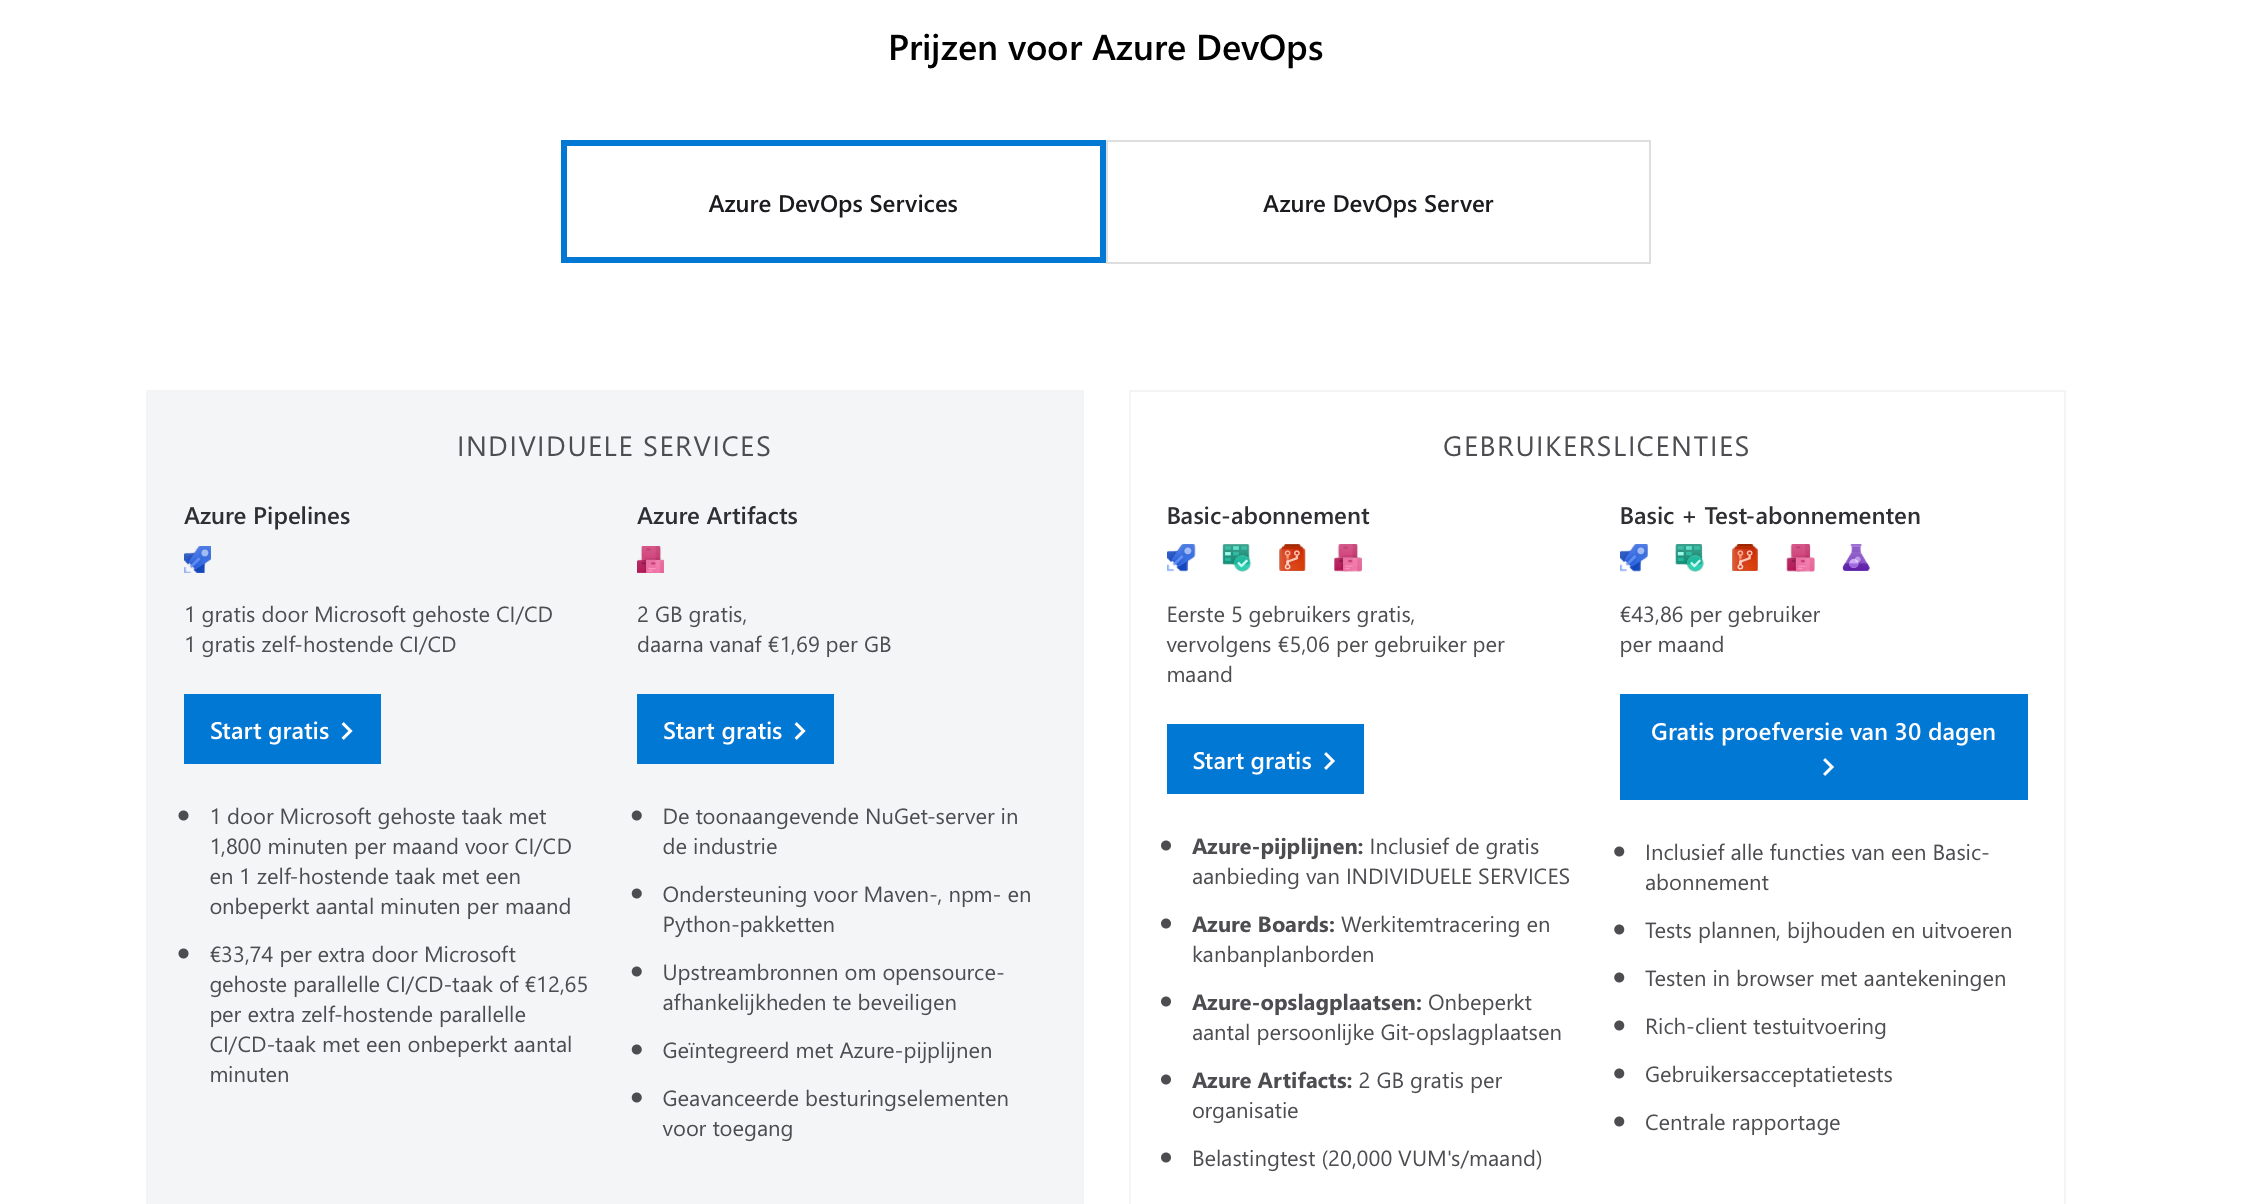
\includegraphics[width=\linewidth]{/Users/kenzie/Documents/HoGent/Bachelorproef/Images/Azure_DO_money.png}
    \caption{Prijzen van Azure DevOps. \href{https://azure.microsoft.com/nl-nl/pricing/details/devops/azure-devops-services/}{Afbeelding van Azure DeVops website}. Figuur toont de prijzen voor Azure DeVops op een beknopte manier.}
    \label{fig:A_DO_Money}
\end{figure}

\section{Google Cloud}
\label{sec:googlecloud}
Google Cloud Platform (GCP) is gelanceerd in April 2008. Het draaide des tijds in dezelfde datacenters als ‘google search’, ‘youtube’ en ‘gmail’. Het was slechts in 2011 dat GCP beschikbaar was voor het brede publiek. GCP is een onderdeel van de Google Cloud. Google Cloud biedt een enorme serie van producten aan waarvan GCP maar een klein onderdeel is. GCP specifiek, biedt ‘infrastructure as a service’ (IaaS), ‘platform as a service’ (PaaS) en ‘serverless computing’ aan. 

Omdat het doel van dit onderzoek specifiek de ondersteuning voor CI/CD vergelijken is, wordt er hier een specifiek onderdeel van GCP bekeken. De ‘Cloud Developper Tools’. Onder deze categorie vallen er een aantal zeer interessante hulpmiddelen. Hier vindt men onder andere ‘Cloud Build’, ‘Cloud-SDK’, ‘Tools voor Powershell’, ‘Tools voor Visual Studio’, enz.

Cloud Build is Google zijn antwoord op een volledige geautomatiseerde CI/CD pipeline. Het is dan ook volledig mede met de moderne vereisten. Met Google Cloud Build (GCB) is een organisatie instaat om snel en gemakkelijk een volledige pijpleiding te configureren. Het gelijkt dan ook op Azure DevOps.

GCB werkt hoofdzakelijk met Git en GitHub om een pijpleiding te bouwen. Google heeft ook zijn eigen ‘Cloud repository service’ die naadloos integreert met GCB, maar deze is helaas betalend. Daarom is het gebruik van Git met GitHub een beter en goedkoper alternatief. Aangezien deze ook perfect integreren met GCB en omdat Git wijdverspreid en simpel in gebruik is. Een organisatie kan dan configureren op GCB dat op het moment van een code update, automatisch een compileer pipeline wordt gestart. Om GCB te laten weten wat er specifiek moet worden uitgevoerd, moet er op de GitHub repository een YAML-bestand voorzien worden waarin regels moeten worden gedefinieerd. Dit maakt het gemakkelijk om snel aanpassingen te maken.

De pipeline op GCB werkt op basis van Docker images. Deze worden in de 'cloudbuild.yml' gedefinieerd. Ook wordt er per Docker container gedefinieerd wat er moet worden uitgevoerd in de vorm van commando’s, script, enz. Dit maakt het mogelijk dat iedere stap in het CI gedeelte van de pipeline volledig kan worden aangepast naar de noden van de organisatie. Zo kan de organisatie beslissen om voor gemaakte containers te gebruiken van de ‘DockerHub’ pagina. Ook kan de organisatie zelf containers maken met aangepaste scripts om bijvoorbeeld in lokale omgevingen testen uit te voeren. GCB kan dus in een hybride opstelling geïmplementeerd worden. Wat ook de bedoeling zou zijn aangezien dit de use case van Aucxis is. Daarnaast biedt GCB ook de mogelijkheid om de gecompileerde code rechtstreeks vanuit Google Cloud beschikbaar te maken voor verdere verdeling.

Met behulp van deze containers kunnen dan functionele testen worden uitgevoerd op de gecompileerde code. Het programma kan dan op basis van de uitkomst van deze uitgevoerde taak, naar de volgende stap zijn wachtrij worden geplaatst. Hier kan de volgende taak starten. GCB genereert rapporten en statistieken van de uitgevoerde taken zodanig dat de gebruiker van het platform inzicht kan krijgen in de uitgevoerde taken.

De compileer en uitvoer-tijden van GCB zijn zeer goed aangezien het platform automatisch schaalt naarmate er meer rekwesten tegelijk worden verstuurd. Dit maakt mogelijk dat verschillende programmeurs tegelijk aan hetzelfde project werken of aan meerdere projecten tegelijk. Ook biedt GCB de mogelijkheid om redundantie te voorzien. GCB maakt het mogelijk om naar andere Cloud platformen uit te rollen of zelfs om de werklast te verdelen over verschillende Cloud platformen. Dit is mogelijk door gebruik te maken van Tekton. Tekton is een open-source framework voor Kubernetes. Dit maakt het mogelijk dat een organisatie over verschillende Cloud platformen heen kan werken. Kubernetes is een clustering hypervisor voor Docker containers. Tekton zou een goede oplossing kunnen zijn voor CI/CD in de Cloud maar valt hier buiten beschouwen vermits het doel de verschillende aanbiedingen van de Cloud platformen vergelijken is.

De prijzen in Google Cloud worden berekend zoals bij ieder moderne Cloud aanbieder. De gebruiker betaald wat hij verbruikt. De volgende \emph{figuur~\ref{fig:GCP_BC_money}} moet dienen om een beeld te vormen over wat men kan verwachten te betalen voor het gebruik van GCB. Dit zonder netwerk kosten voor het transfereren van gegevens. Er wordt ook niks in rekening gebracht voor zaken die in een wachtrij staan of pipelines die niet worden gebruikt. De Google Cloud Developper Tools hebben een voordeel. Een groot deel van de hulpmiddelen voor ondersteuning met het platform zijn gratis. Er zijn ook weinig hulpmiddelen van derden nodig om de gewilde functionaliteit te bereiken.

\begin{figure}[!htbp]
    \centering
    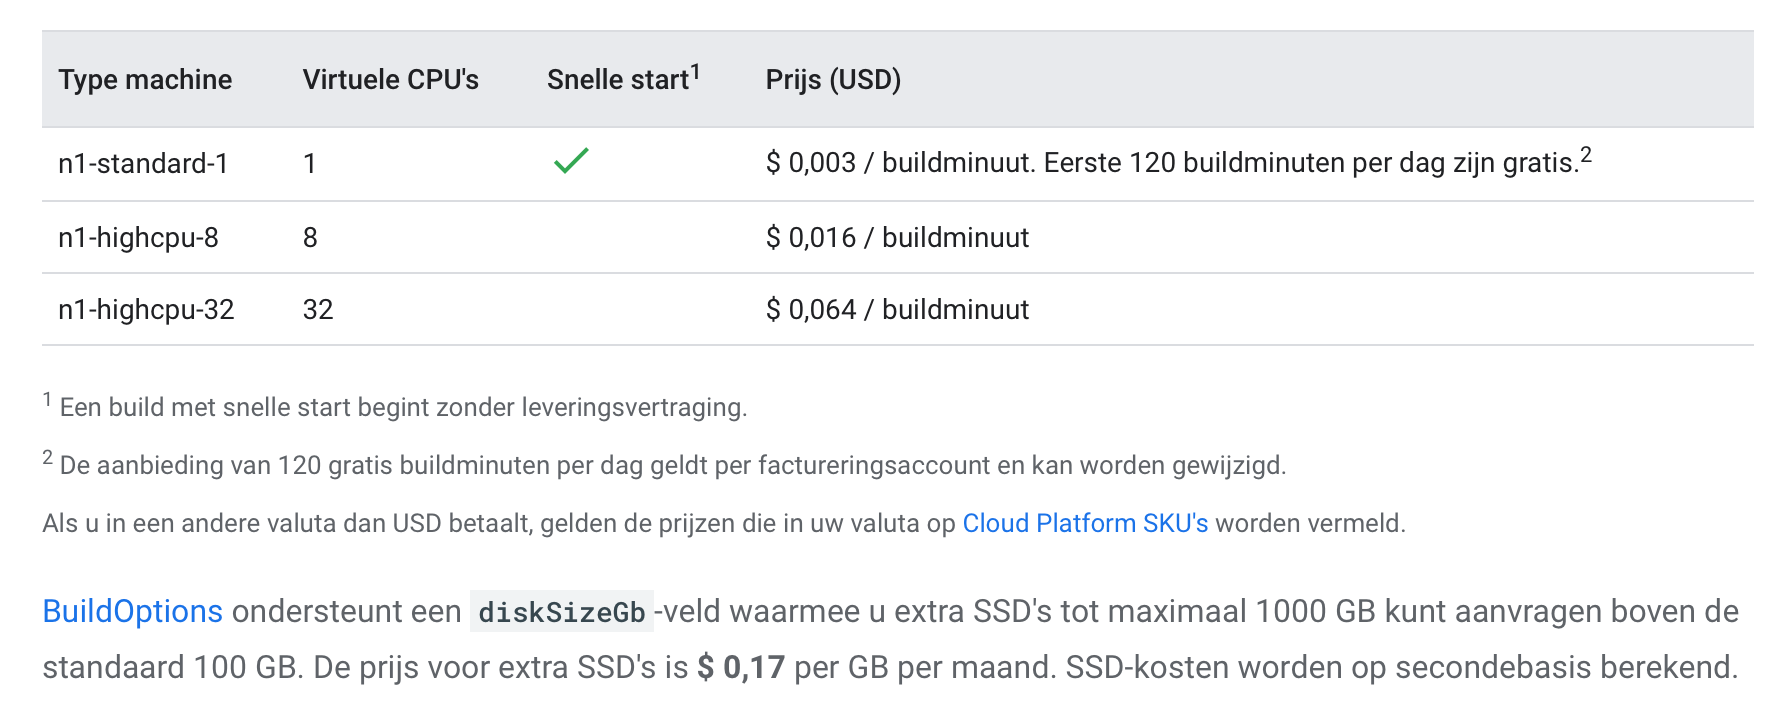
\includegraphics[width=\linewidth]{/Users/kenzie/Documents/HoGent/Bachelorproef/Images/gcp_bc_money.png}
    \caption{GCB prijzen. \href{https://cloud.google.com/cloud-build/pricing}{Figuur van Google Cloud website}. Figuur toont de prijzen voor Google Cloud Platform op een beknopte manier.}
    \label{fig:GCP_BC_money}
\end{figure}

Met andere woorden is GCB dus een volwaardig alternatief voor Azure DevOps. Er is ondersteuning voor verschillende tools, biedt uitgebreide functionaliteiten aan en bovendien adverteert Google dat het gemakkelijk samenwerkt met andere Cloud platformen. Het zei door het gebruik van Tekton. Andere Cloud platformen ondersteunen dit ongetwijfeld ook. Alleen wordt er niet mee reclame gemaakt zoals bij GCP. Daarnaast is het ook relatief simpel in gebruik door dat GCB gebruikmaakt van Docker containers voor te compileren.

\section{Amazon Web Services}
\label{sec:amazonaws}
Amazon web services (AWS) is gelanceerd in 2006. Gedurende lange tijd heeft Amazon stukken van hun datacenter verhuurd aan het brede publiek. Tegenwoordig kan een gebruiker op AWS een Cloud computer samenstellen juist zoals een gewone server zou worden samengesteld. Het is maar in recente tijden dat Amazon zich meer beginnen focussen is op services voor de gebruiker. Zo bevat AWS nu meer dan 212 services en producten. Bijvoorbeeld: virtuele computerkracht, netwerking, opslag in de Cloud, databases, statistieken, programma services, uitrol op de Cloud, beheer van bepaalde zaken, ontwikkelingshulpmiddelen en hulpmiddelen voor 'Internet Of Things' (IoT). De populairste tegenwoordig zijn 'Amazon Elastic Compute Cloud' (EC2) en 'Amazon Simple Storage Service' (Amazon S3). Deze laatste zijn in feite Cloud computerkracht en opslag voor verschillende doeleindes. Deze zijn volledig schaalbaar en zijn gratis om te creëren.

Ondanks dit groot aanbod resteert er toch nog altijd de vraag hoe het zit met de huidige prestatie van Amazon datacenters over de hele wereld. Zeker na het lezen van deze paper \autocite{Jackson2010}. Voor dit onderzoek is er ijverig gezocht naar recentere prestatie onderzoeken maar zonder resultaat. Er kan alleen maar worden afgegaan van Amazon zijn website.

Al deze producten en services maken het niet gemakkelijk voor een gebruiker om snel te weten welke producten voor hem geschikt zijn. Ook in dit onderzoek is er vastgesteld dat het lastig is om een duidelijk beeld te krijgen wat er allemaal mogelijk is. Dat terzijde, heeft Amazon toch een specifiek aanbod om CI/CD te implementeren op hun Cloud platform. Zo heeft Amazon, AWS CodePipeline. Dit is een service waarbij de gebruiker of organisatie via het web portaal gemakkelijk een CI/CD pijpleiding kan definiëren. Deze is volledig aanpasbaar naar de noden van de gebruiker. AWS CodePipeline gebruikt AWS CodeBuild voor de compilatie en het testen van projecten in CI/CD en AWS CodeDeploy voor het automatische uitrollen van projecten.

Zoals alle grote Cloud platformen ondersteund AWS CodePipeline ook het gebruik van Git en GitHub. De gebruiker hoeft dus geen speciale zaken te doen. Amazon heeft ook zijn eigen Cloud repositories voor code op te bewaren. Deze zijn ook gebaseerd op Git. Het zijn eigenlijk privé Git repositories die door Amazon worden aangeboden. Het gebruik verschilt niet tussen GitHub en Amazon zijn privé Git servers. De gebruiker kan gemakkelijk via het web portaal de gewenste Git-projecten toevoegen aan AWS CodePipeline.

AWS CodeBuild is een CI service die code compileert, testen uitvoert en als resultaat software oplevert. AWS CodeBuild is speciaal omdat er geen nood is om zelf de server infrastructuur te configureren voor de compilatie van code. AWS CodeBuild doet dit allemaal voor de gebruiker en schaalt mede naarmate de belasting of het project groter wordt. AWS CodeBuild maakt gebruik van voorverpakte compileer omgevingen maar de gebruiker heeft wel de mogelijkheid om zelf zijn compileer omgevingen te configureren. Dit maakt mogelijk dat de pipeline volledig aan te passen is naar de noden van de gebruiker. 

Zodat Amazon weet wat voor compileer omgeving er moet worden gebouwd, moet de gebruiker aan de project folder een BuildSpec.yml toevoegen waarin staat welke compileer engine er gebruikt moet worden met welke files. 

Dit kan ook worden gedefinieerd in het web portaal zodanig dat de gebruiker niet de hele tijd broncode moet updaten bij wijzigingen aan de configuratie. Ook heeft AWS CodeBuild een voordeel. Na de compilatie en testen geslaagd zijn, kan er direct een zip gemaakt worden die dan downloadbaar is van Amazon zijn Cloud opslag. AWS CodeBuild zijn prijzen worden op dezelfde manier berekend als Google Cloud Build. Er wordt betaald per minuut dat er computerkracht gebruikt wordt. Zie de \emph{figuur~\ref{fig:AWS_CB_money}} en \emph{figuur~\ref{fig:AWS_CB_money2}}

\begin{figure}[!htbp]
    \centering
    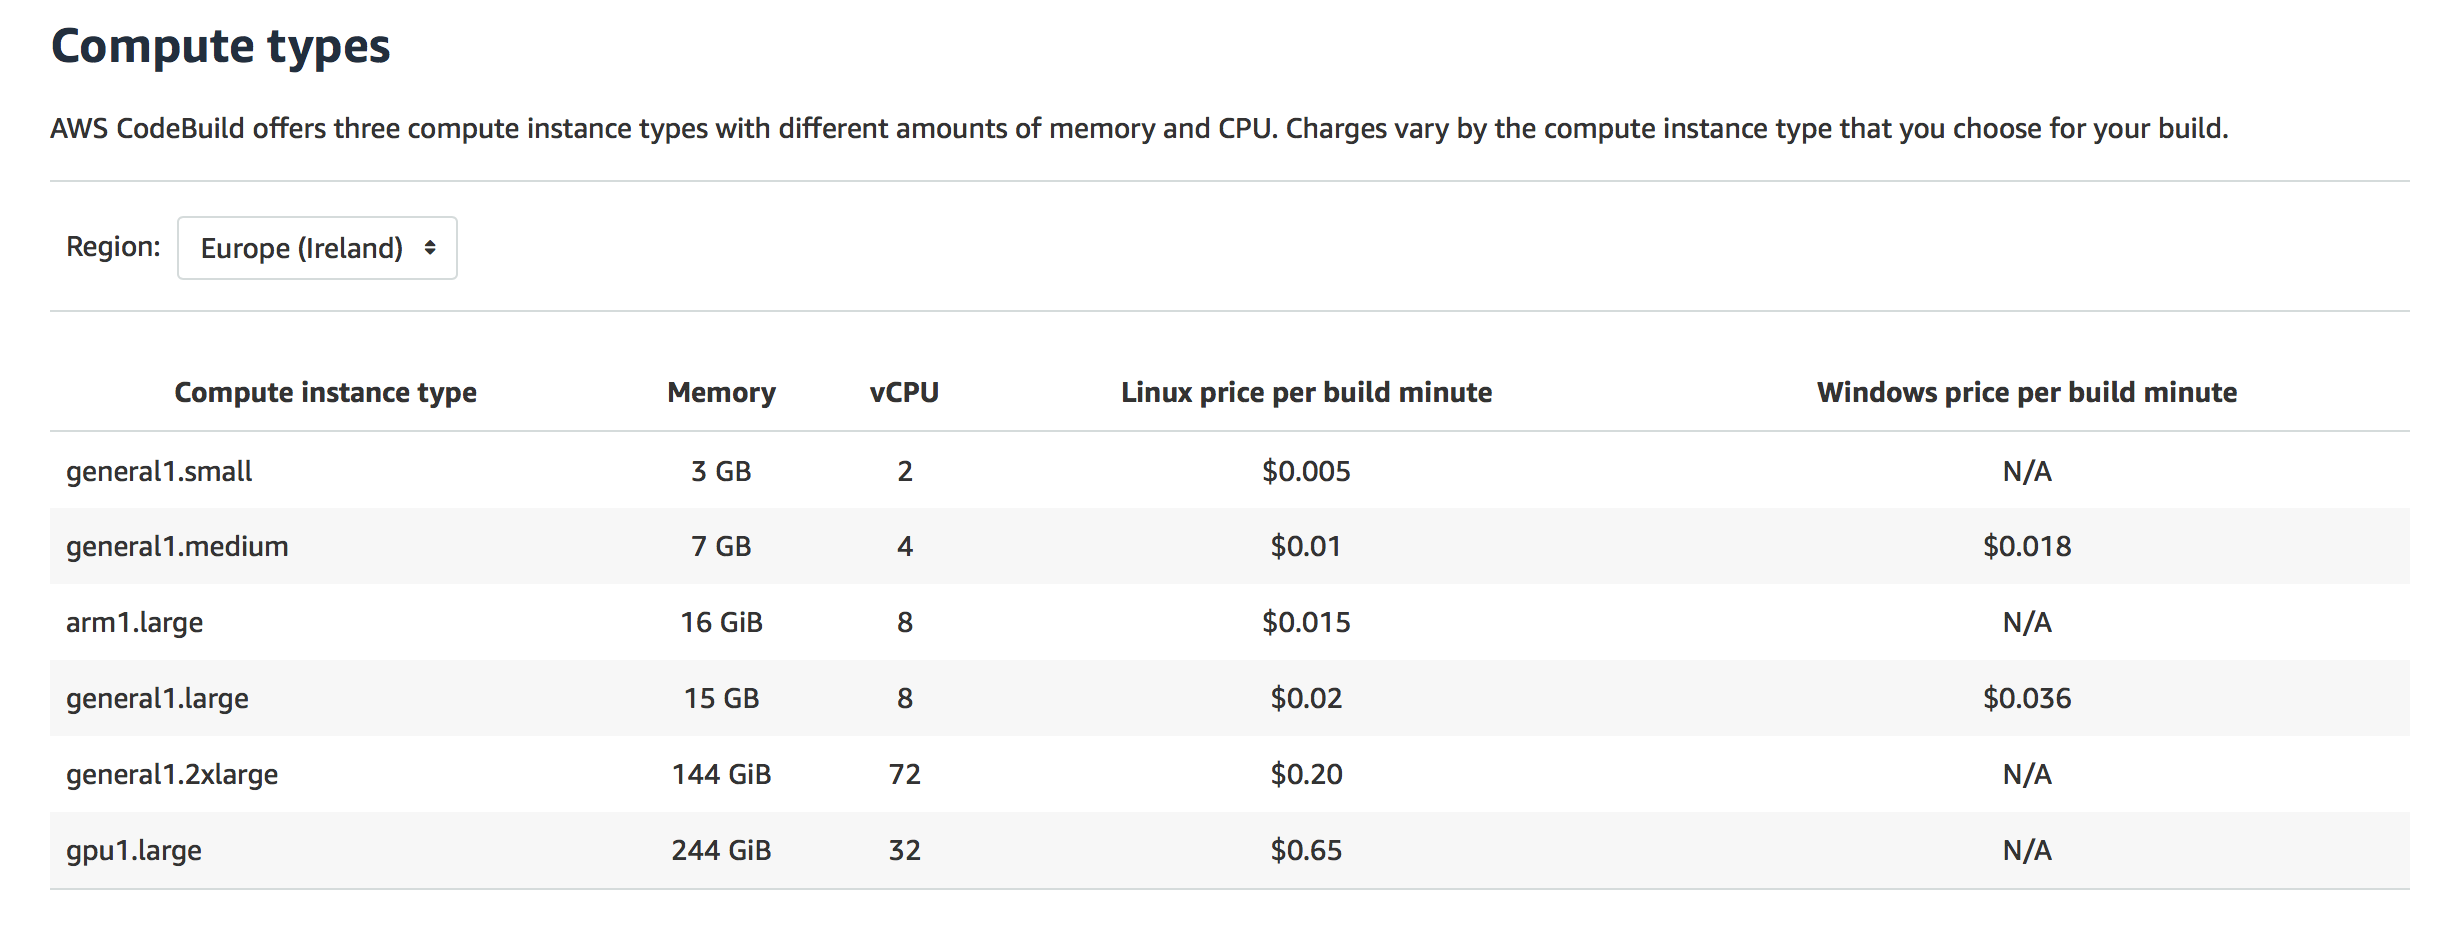
\includegraphics[width=\linewidth]{/Users/kenzie/Documents/HoGent/Bachelorproef/Images/AWS_CB_money.png}
    \caption{ \href{prijzen AWS computekracht.}{Figuur van AWS website}. Figuur toont de prijzen van AWS per rekenkracht, OS en verstreken minuut.}
    \label{fig:AWS_CB_money}
\end{figure}
\begin{figure}[!htbp]
    \centering
    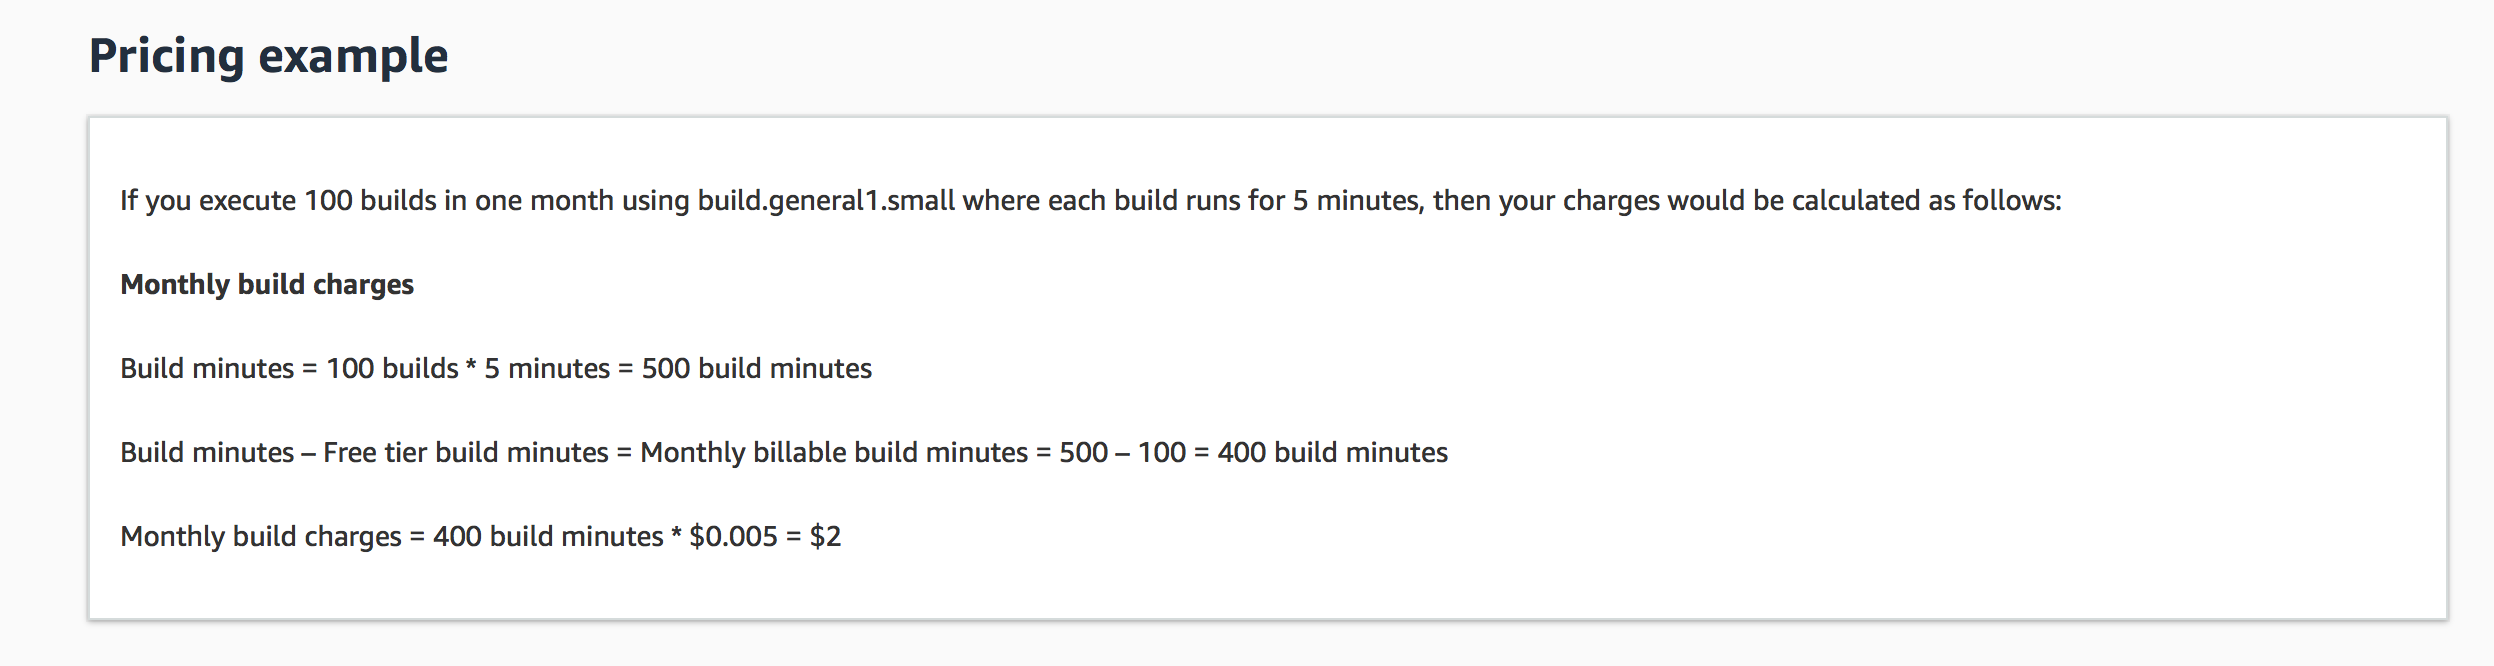
\includegraphics[width=\linewidth]{/Users/kenzie/Documents/HoGent/Bachelorproef/Images/AWS_CB_money2.png}
    \caption{compileer prijzen AWS.\href{}{Figuur van AWS website}. Figuur toont berekening van prijzen per compileer minuut voor AWS.}
    \label{fig:AWS_CB_money2}
\end{figure}

Een klein detail dat maar zichtbaar was bij het bekijken van de prijzenstelsels. De gebruiker heeft de mogelijkheid om een besturingssysteem (OS) te kiezen bij het aanmaken van een AWS CodeBuild pipeline. Dit onderzoek heeft vastgesteld dat een Windows OS wel beschikbaar is maar niet in iedere datacenter locatie. Vaak is die optie ook duurder dan de Linux variant. Dit kan eventueel problemen veroorzaken met Windows specifieke voorbeelden. Ook is het moeilijk om informatie te vinden over hoe de gebruiker nu juist zelf een aangepaste compileer omgeving definieert. 

AWS CodeDeploy is het CD gedeelte van de AWS CodePipeline. Het is volledige te beheren en aanpasbaar naar de noden van de gebruiker. Zo is het mogelijk om rechtstreeks vanuit de pipeline uit te rollen naar eender welke Amazon Cloud service of naar lokale omgevingen. Aangezien het mogelijk is om een zip met de software in te downloaden is het ook gemakkelijk te integreren met bestaande uitrol tools of procedures. Deze feature is ook niet gratis. Volgende \emph{figuur~\ref{fig:AWS_CD_money}} toont dit aan. Amazon rekent per update van een instantie een prijs aan. Daarbovenop moet er ook nog betaald worden voor de verbruikte opslag.

\begin{figure}[!htbp]
    \centering
    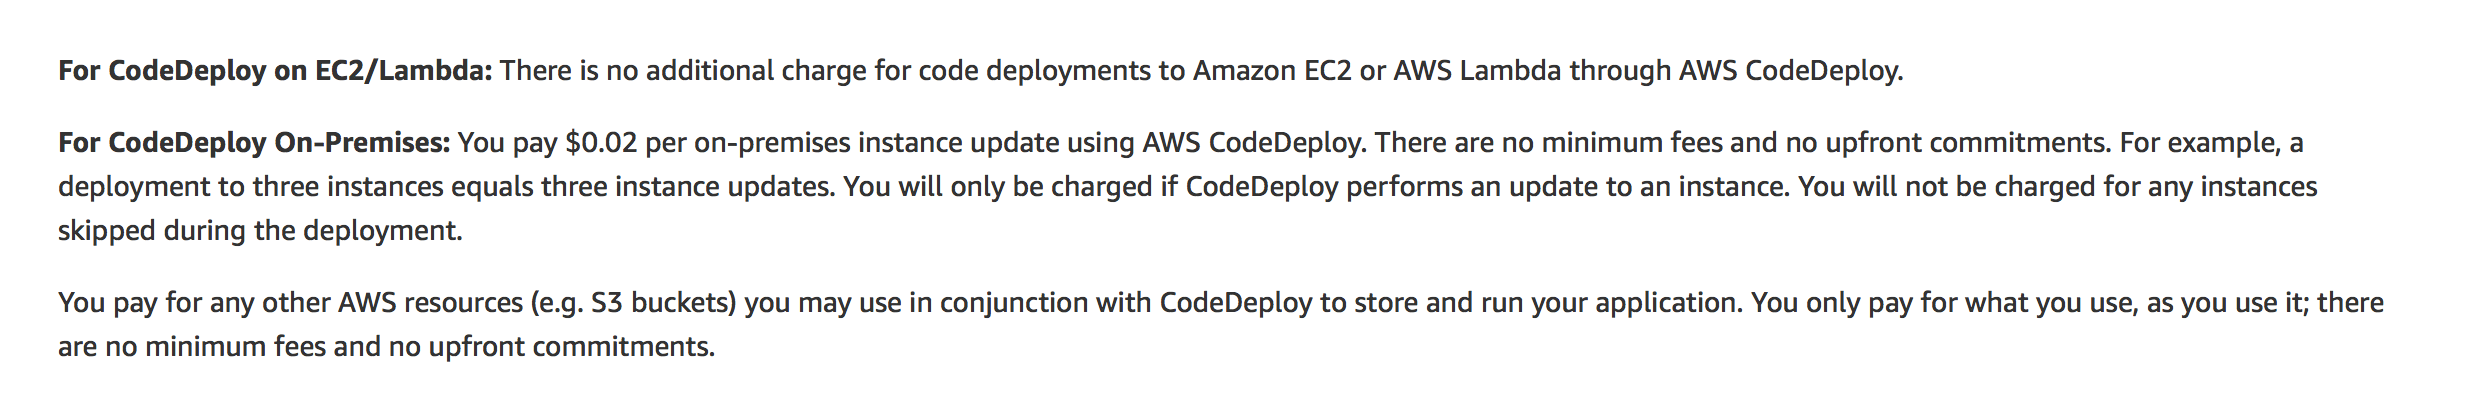
\includegraphics[width=\linewidth]{/Users/kenzie/Documents/HoGent/Bachelorproef/Images/AWS_CD_money.png}
    \caption{extra kosten. \href{}{Figuur van AWS website}. Figuur toont prijs voor opslag op AWS.}
    \label{fig:AWS_CD_money}
\end{figure}

Naast een hele serie ontwikkelingshulpmiddelen heeft Amazon ook hulpmiddelen toegevoegd om gedetailleerde rapporten en analyses te genereren van de uitgevoerde taken op AWS CodePipeline. Dit geeft  de gebruiker goede inzichten in wat er juist allemaal gebeurt en verkeerd loopt. Ook kan de gebruiker op basis van foutmeldingen of status rapporten, bepaalde acties instellen en laten uitvoeren.

Het zou mogelijk zijn om met AWS de gewilde functionaliteit te realiseren. Het zal wel zeer arbeid intensief zijn aangezien informatie over een aangepaste compilatie omgeving moeilijk te vinden is. Ook is het een stuk duurder. Dit onderzoek heeft ook vastgesteld dat Amazon een hele reeks van producten heeft waardoor het soms moeilijk is om door het bos de bomen te zien. Ook de prestatie van het platform blijft een vraagteken door de paper \autocite{Jackson2010}.

\section{IBM Cloud}
\label{sec:ibmcloud}
IBM Cloud is mogelijk een van de oudere Cloud platformen. Nog voor de term Cloud veel gebruikt werd. IBM was al vroeg bezig met het idee om hardware open te stellen om dan meerdere machines of services op te laten draaien. In 1972 heeft IBM de eerste stappen gezet naar IaaS door voor hun mainframe een hypervisor te bouwen die toestond dat er meerdere instanties van een besturingssysteem op hetzelfde systeem draaide (VM’s). Dit is dan later geëvolueerd naar een meer typische Cloud infrastructuur. IBM heeft in de vroege jaren van hun Cloud systeem, vooral hardware voorzien aan klanten. De zo genoemde privé Cloud. In 2007 werden dan de eerste stappen gezet naar de typisch Cloud infrastructuur door het verhuur van rekenkracht vanuit hun datacenters met hun hardware. 

Heden ten dage is IBM Cloud een stuk uitgebreider. Het valt onder te verdelen in drie grote categorieën. 'SmartCloud Foundation', 'SmartCloud Service's en 'SmartCloud Solutions'. Volgens IBM is het hun bedoeling om de gaten in het aanbod van andere Cloud platform aanbieders op te vullen.

'SmartCloud Foundation' is een serie producten die privé Cloud en Hybride Cloud mogelijk moeten maken. Het biedt de infrastructuur, beheer, beveiliging, hardware en integratie aan. 'SmartCloud Services' zijn dan de verschillende hulpmiddelen om dit te bereiken of te gebruiken. (Iaas of PaaS.) 'SmartCloud Solutions' is dan meer een pakket dat samenwerking, statistieken enz. moet mogelijk maken binnen de services en aanbiedingen van IBM.

Ook IBM Cloud heeft producten om een CI/CD pipeline te maken. Al is er toch een addertje onder het gras. IBM Cloud voorziet infrastructuur om vooral CD te kunnen realiseren. Dit met mogelijkheden om de infrastructuur te definiëren. Hulpmiddelen om de uitrol te beheren en te analyseren. Dit alles kan worden gecontroleerd, zoals alle andere Cloud platform aanbieders, door middel van een speciaal ontwikkelde command line interface (CLI) of door hun web portaal. Voor CI biedt IBM niks specifiek aan. Er bestaat wel de mogelijkheid om het Tekton framework te gebruiken op de Cloud infrastructuur van IBM maar dat kan bij ieder Cloud platform. Dit framework valt ook buiten de scope van dit onderzoek.

Op basis van hun producten en services die ze aanbieden valt IBM Cloud uit de boot. Het zou zeer omslachtig zijn om IBM Cloud te gebruiken voor een Microsoft georiënteerde pipeline. Aangezien er geen specifieke compileer technieken aanwezig zijn. Naast het Tekton framework. Ook is de prestatie van de IBM-datacenters niet slecht. Het zijn speciaal ontworpen centers met eigen hardware en voorzieningen van IBM. Wat wel blijkt uit onderzoek van de ontwikkelingshulpmiddelen van IBM Cloud, is dat IBM zich inzet om gemakkelijk te gebruiken hulpmiddelen te ontwikkelen die weinig moeite kosten om te implementeren en te configureren. Ook hebben ze als enige specifiek een Cloud aanbod voor Apple georiënteerde applicaties.

\section{Andere}
\label{sec:oracledigitalocean}
Naast de alom bekende giganten zoals Azure, Google Cloud, IBM Cloud en AWS zijn er nog een aantal andere Cloud platform aanbieders. Zo bestaat er nog Oracle Cloud en Digital Ocean. Er bestaan waarschijnlijk nog wel maar deze laat dit onderzoek buiten beschouwing.

Oracle Cloud zijn aanbod van producten en services liggen vooral in vier categorieën. IaaS, PaaS, 'Software as a Service' (SaaS) en 'Data as a Service'. Oracle Cloud hun aanbod is hoofdzakelijk hetzelfde als alle andere Cloud platformen. Juist zoals IBM Cloud heeft Oracle hun eigen hardware en eigen datacenters. Oracle Cloud biedt oplossingen en producten aan om DevOps te realiseren maar deze zijn vooral gefocust op het Java platform. Om deze reden valt ook Oracle Cloud uit de boot. Aangezien we in dit onderzoek trachten om een Microsoft georiënteerde pipeline te realiseren. Het is wel mogelijk door gebruik te maken van het Tekton Framework. Maar dit laten we buiten beschouwing in dit onderzoek.

Digital Ocean is een Cloud platform speciaal gemaakt voor ontwikkelaars. Het Cloud platform is een van de jongere spelers tussen de Cloud platformen. Digital Ocean is opgericht in 2011. Hun doel is om een omgeving aan te bieden aan ontwikkelaars waarin programmeurs gemakkelijk kunnen ontwikkelen en testen. Ook tracht Digital Ocean om deze omgeving open te stellen voor productie door het zeer gemakkelijk te maken om services en applicatie schaalbaar te maken op hun platform. Digital Ocean heeft jammer genoeg geen specifiek CI/CD mogelijkheid. Het zou wel mogelijk zijn met het Tekton framework aangezien Digital Ocean Kubernetes ondersteund. Voor deze redenen valt Digital Ocean ook buiten de boot.

\section{Gebruiksvriendelijkheid}
\label{sec:KandidaatSelectie}
Naast de kandidaat selectie op productaanbod en prijs, wil dit onderzoek ook de gebruiksvriendelijkheid in acht nemen. Hiervoor is er een simpele Java applicatie gebruikt. Alle Cloud platformen bieden startershandleidingen aan voor het opzetten van een CI-pipeline voor Java op hun platform. Het doel van deze snelle test is om als eindresultaat een werkende Java JAR te hebben. Ook werd er bijgehouden hoelang het duurde om een pijpleiding te configureren om beter een idee te krijgen van hoe gebruiksvriendelijk het Cloud platform werkelijk is. 

De Java Applicatie bestaat uit een hoofdklasse en een testklasse. De hoofdklasse, ‘MessageUtil’ bevat een variabele voor een bericht te bewaren en vier methodes. De eerste methode is een constructor voor het aanmaken van een ‘MessageUtil’ object met een meegegeven bericht. De tweede methode print dit bericht. In de derde methode wordt er een toevoegsel aan dit bericht gevoegd. Ook wordt het geheel geprint. De laatste methode is een uitvoerbare methode die een ‘MessageUtil’ object maakt en de twee print methodes uitvoert. De code voor ‘MessageUtil.java’ wordt afgebeeld in \emph{figuur~\ref{code:messageutilj}}. 

De testklasse ‘TestMessageUtil’ bevat twee testen voor de print methodes. \emph{Figuur~\ref{code:messageutiltestj}}  toont de code voor dit Javabestand.

\lstset{
    language=java,
    breaklines=true,
    frame=single,
    commentstyle=\color{mygreen},
    keywordstyle=\color{blue},
    numberstyle=\tiny\color{mygray},
    stringstyle=\color{mymauve},
    captionpos=b,
    caption={Java bestand MessageUtil.java. Hoofd klasse van de applicatie \emph{MessageUtil}},
    label=code:messageutilj
}
\begin{lstlisting}
public class MessageUtil {
private String message;

public MessageUtil(String message) {
this.message = message;
}

public String printMessage() {
System.out.println(message);
return message;
}

public String salutationMessage() {
message = "Hi!" + message;
System.out.println(message);
return message;
}

public static void main(String[] args) {
MessageUtil mu = new MessageUtil("Aucxis ...");
mu.printMessage();
mu.salutationMessage();
}
}
\end{lstlisting}

\lstset{
    language=java,
    caption={Java Test klasse MessageUtilTest.java, voor het testen van \emph{MessageUtil~\ref{code:messageutilj}}.},
    label=code:messageutiltestj
}
\begin{lstlisting}
import org.junit.Test;
import org.junit.Ignore;
import static org.junit.Assert.assertEquals;

public class TestMessageUtil {

String message = "Robert";    
MessageUtil messageUtil = new MessageUtil(message);

@Test
public void testPrintMessage() {      
System.out.println("Inside testPrintMessage()");     
assertEquals(message,messageUtil.printMessage());
}

@Test
public void testSalutationMessage() {
System.out.println("Inside testSalutationMessage()");
message = "Hi!" + "Robert";
assertEquals(message,messageUtil.salutationMessage());
}
}
\end{lstlisting}

Deze Javabestanden worden op alle Cloud platformen gecompileerd aan de hand van de Maven compiler. Om de compiler te vertellen wat er moet gebeuren tijdens de compilatie van de Javabestanden, moet er een Xml-bestand worden aangemaakt waarin deze opties gedefinieerd staan. Deze ‘pom.xml’ wordt afgebeeld door \emph{figuur~\ref{code:pom}}. Hierin staat dat de meegeleverde Junit testen moeten worden uitgevoerd. Ook wordt er gedefinieerd dat de Java applicatie moet worden gecompileerd tot een JAR-bestand.

\lstset{
    language=XML,
    caption={XML-bestand voor de Maven compiler. Definieert stappen voor het compileren van een java applicatie.},
    label=code:pom
}
\begin{lstlisting}
<project xmlns="http://maven.apache.org/POM/4.0.0" 
xmlns:xsi="http://www.w3.org/2001/XMLSchema-instance"
xsi:schemaLocation="http://maven.apache.org/POM/4.0.0 http://maven.apache.org/maven-v4_0_0.xsd">
<modelVersion>4.0.0</modelVersion>
<groupId>org.example</groupId>
<artifactId>messageUtil</artifactId>
<version>1.0</version>
<packaging>jar</packaging>
<name>Message Utility Java Sample App</name>
<dependencies>
<dependency>
<groupId>junit</groupId>
<artifactId>junit</artifactId>
<version>4.11</version>
<scope>test</scope>
</dependency>	
</dependencies>
<build>
<plugins>
<plugin>
<groupId>org.apache.maven.plugins</groupId>
<artifactId>maven-jar-plugin</artifactId>
<version>3.1.0</version>
<configuration>
<archive>
<manifest>
<addClasspath>true</addClasspath>
<classpathPrefix>lib/</classpathPrefix>
<mainClass>MessageUtil</mainClass>
</manifest>
</archive>
</configuration>
</plugin>
</plugins>
</build>
</project>
\end{lstlisting}

Deze bestanden zijn toegevoegd aan een folder die de structuur hanteert uit \emph{figuur~\ref{code:treejava}}. Deze hoofdmap is dan geïnitialiseerd als een Git repository. Ook is er een gitignore aangemaakt. Deze Java applicatie is het startpunt voor alle testen voor gebruiksvriendelijkheid op de Cloud platformen. Op deze manier is er geprobeerd om op basis van eventuele verschillen een geschikte kandidaat te selecteren voor een Proof Of Concept. In de volgende secties~\ref{sec:JAA}, ~\ref{sec:JGCP} \& ~\ref{sec:JAD} wordt kort de werkwijze beschreven. Hier wordt de ‘hoe’ minder aangehaald omdat dit in de handleiding beschreven staat.

\lstset{
    language=bash,
    caption={Output van het tree commando in een java applicatie bestanden structuur.},
    label=code:treejava
}
\begin{lstlisting}
Demo_java_aws/
`--- .gitignore
`--- pom.xml
`--- src
    `--- main
        `--- java
            `--- MessageUtil.java
    `--- test
        `--- java
            `--- TestMessageUtil.java
\end{lstlisting}

\subsection{Java Amazon AWS}
\label{sec:JAA}
Voor de test op Amazon AWS is deze \emph{\href{https://docs.aws.amazon.com/codebuild/latest/userguide/getting-started.html}{handleiding}} gevolgd. Er zijn wel een aantal zaken aangepast geweest om een realistischere opstelling te benaderen. De handleiding begint met het aanmaken van twee S3 Storage Buckets. In dit geval is er gekozen om maar een S3 Storage Bucket aan te maken. Deze zal dienen als een output voor bestanden. Voor de input werd een GitHub repository gebruikt. Vervolgens wordt in de handleiding de applicatie gemaakt. Voor dit experiment is er voor de drie Cloud platformen dezelfde applicatie gebruikt. \emph{Figuur~\ref{code:messageutilj}} toont de hoofdklasse van deze applicatie en \emph{figuur~\ref{code:messageutiltestj}} toont de testklasse van deze applicatie. Vervolgens wordt er in de handleiding een YAML-bestand aangemaakt waarin de verschillende stappen voor het compileren en testen van de applicatie worden gedefinieerd.

Dit YAML-bestand heeft op Amazon AWS de naam ‘buildspec.yml’. \emph{Figuur~\ref{code:buildspec}} toont dit bestand. Over het aanpassen van dit YAML-bestand is er maar weinig informatie te vinden. Ook is het niet helemaal duidelijk hoe er precies een andere virtuele machine moet worden gekozen. Tijdens het uitvoeren van de configuratie is er gebleken dat de documentatie tot verwarring kan lijden. Dit YAML-bestand bevat altijd vier fases waarin een reeks commando’s kunnen worden uitgevoerd. De eerste fase is de ‘install‘ fase. Hier wordt er gedefinieerd wat voor omgeving moet worden gebruikt. In dit geval gebruikt de handleiding ‘corretto11’. Dit is een Linux gebaseerde machine. De tweede fase is de ‘pre-build’ fase. Hierin kunnen er commando’s worden uitgevoerd om de machine voor te bereiden, repositories te kopiëren, enz. In dit geval staat er een echo-commando als plaatsvulling. De derde stap is de ‘build’ stap. Hierin worden de commando’s geschreven die ervoor moeten zorgen dat de applicatie wordt gecompileerd. In een vierde fase, de ‘post-build’ fase, is er de mogelijkheid om nog commando’s uit te voeren na het compileren van de applicatie. Dit is in dit geval ook ongebruikt. Voor een Java applicatie wordt alles door middel van een pom.xml uitgevoerd. \emph{Figuur~\ref{code:pom}} toont dit bestand. Het enige dat dus moet worden gedefinieerd in de ‘buildspec.yml’ is het uitvoeren van een herstel op de Java-bestanden.

\lstset{
    language=bash,
    caption={YAML-bestand voor het configureren van een pijpleiding op Amazon AWS.},
    label=code:buildspec
}
\begin{lstlisting}
version: 0.2

phases:
    install:
    runtime-versions:
        java: corretto11
    pre_build:
        commands:
            - echo Nothing to do in the pre_build phase...
    build:
        commands:
            - echo Build started on `date`
            - mvn install
    post_build:
        commands:
            - echo Build completed on `date`
    artifacts:
    files:
        - target/messageUtil-1.0.jar
\end{lstlisting}

In een volgende stap wordt in de handleiding de pipeline aangemaakt op Amazon AWS. Dit werd volledig gedaan via de online console van Amazon AWS. Een verschil in deze configuratie is het selecteren van een bron voor de broncode. Deze bevind zich nu op GitHub. \emph{Figuur~\ref{fig:aws_java_demo_conf}} toont de gewijzigde configuratie op AWS. Voor alle ander opties is de handleiding gevolgd. Ook de volgende stappen vanuit de handleiding zijn onveranderd gevolgd. Zo werd er als resultaat in de Bucket een Jar-bestand achtergelaten. Deze was zeer gemakkelijk te downloaden om daarna uit te voeren.

\begin{figure}[!htbp]
    \centering
    \includegraphics[width=\linewidth]{/Users/kenzie/Documents/HoGent/Bachelorproef/Images/aws_java_demo_conf.png}
    \caption{BronCode locatie seleceteren op AWS. Deze figuur toont het selecteren van een GitHub repositorie bij het aanmaken van een pipeline op Amazon AWS.}
    \label{fig:aws_java_demo_conf}
\end{figure}

Het volgen van deze handleiding ging niet zonder slag of stoot. Het was in het begin zeer moeilijk om te begrijpen wat ‘buildspec.yml’ nu allemaal kan. Ook heeft Amazon AWS een hele reeks van producten dat het soms moeilijk maakt om te selecteren wat er nu juist nodig is. De tijd die in beslag genomen is in vergelijking met de andere platformen, om de handleiding van het begin tot het einde te volgen wordt getoond in \emph{tabel~\ref{tab:gebruiksvriendelijkheid}}. Hier is ook het opstellen van de applicatie meegerekend en ook het uitvoeren van het resulterende Jar-bestand.

\subsection{Java Google Cloud Platform}
\label{sec:JGCP}
Voor Google Cloud Code Build is volgende \emph{\href{https://cloud.google.com/cloud-build/docs/building/build-java}{handleiding} }gebruikt geweest. Al snel bleek bij het begin van de handleiding dat er geen manier was om via een online console een pipeline te configureren. De pipeline en de verschillende logs kunnen wel bekeken worden op het portaal. Er bestaat een mogelijkheid om in de console een terminal te openen waarin Google Cloud CLI geïnstalleerd staat. Hiermee kan de gebruiker alle producten beheren op het platform. Om een pijpleiding aan te maken van op een lokale computer, moet eerst de \emph{\href{https://cloud.google.com/sdk?hl=nl}{Google Cloud CLI}} worden geïnstalleerd. Deze CLI is beschikbaar op ieder besturingssysteem en staat de gebruiker toe om alle services en producten van GCP aan te sturen en te beheren. De installatie ervan is eenvoudig. Zeker met behulp van de \emph{\href{https://cloud.google.com/sdk/docs/downloads-versioned-archives?hl=nl}{documentatie}} van Google zelf. Ook moet er een recente versie van Python beschikbaar zijn op de gebruiker zijn computer. Na deze te hebben geïnstalleerd  moet het Google Cloud account geconnecteerd worden aan de CLI. Deze \emph{\href{https://cloud.google.com/sdk/docs/initializing?hl=nl}{documentatie}} legt dit zorgvuldig uit.

Daarna gaat de handleiding verder met het definiëren van een YAML-bestand voor de configuratie van de pipeline. Bij Google Cloud noemt dit bestand ‘cloudbuild.yml’. \emph{Figuur~\ref{code:cloudbuildj}} toont het gebruikte bestand voor dit geval. In deze configuratie kunnen er zoveel stappen worden gedefinieerd als de gebruiker wenst. In dit geval zijn er slechts twee stappen gedefinieerd. In een eerste stap wordt de code getest door middel van het test commando op een Maven Docker container. In een tweede stap wordt door middel van dezelfde machine de applicatie gecompileerd tot een Jar-bestand. In een aanvullende stap wordt deze Jar geüpload naar een Storage Bucket op Google Cloud. Een Storage Bucket kan worden gecreëerd door middel van de console. De gebruiker moet enkel een naam ingeven. Hierna is er het commando ‘glcoud submit’ uitgevoerd om deze pijpleiding uit te voeren. 

\lstset{
    language=bash,
    caption={YAML-bestand voor het configureren van een pijpleiding voor java op Google Cloud.},
    label=code:cloudbuildj
}
\begin{lstlisting}
steps:
    - name: maven:3-jdk-8
        entrypoint: mvn
        args: ['test']
    - name: maven:3-jdk-8
        entrypoint: mvn
        args: ['package','-Dmaven.test.skip=true']
    artifacts:
    objects:
        location: 'gs://output-bucket-codebuild/target/'
        paths: ['/workspace/target/messageUtil-1.0.jar']
\end{lstlisting}

Dit hele proces was vrijwel pijnloos. Ook de extra documentatie voor het aanmaken van Storage Buckets, het uploaden van artifacten en het installeren van Google Cloud Cli, was gemakkelijk te vinden. Het gecompileerde Jar-bestand was gemakkelijk te downloaden van de Stroage op Google Cloud. De tijd die in beslag genomen is in vergelijking met de andere platformen, om de handleiding van het begin tot het einde te volgen wordt getoond in \emph{tabel~\ref{tab:gebruiksvriendelijkheid}}. Hier is ook het opstellen van de applicatie meegerekend en ook het uitvoeren van het resulterende Jar-bestand. Deze configuratie ging vlot door het gemakkelijk vinden van de benodigde informatie en de intuïtieve configuratie bestanden.

\subsection{Java Azure DevOps}
\label{sec:JAD}
Voor deze opstelling is deze \emph{\href{https://docs.microsoft.com/en-us/azure/devops/pipelines/ecosystems/java?view=azure-devops}{handleiding}} gebruikt geweest. Vooraleer deze handleiding kon worden gevolgd, is er eerst een nieuwe organisatie aangemaakt geweest in Azure DevOps. Binnen deze organisatie is er dan een nieuw project aangemaakt geweest om de pipelines in te configureren. Zo een Azure DevOps project bevat een hele serie producten en services om ontwikkelaars en organisaties te helpen in het softwareontwikkelingsproces. Ook is zo een project handig omdat het net zoals de andere Cloud platformen, alle aanrekeningen en producten stopzet bij het verwijderen.

Verder moest er ook een GitHub repository bestaan om deze handleiding te kunnen starten. Deze repository bevat de Java applicatie met de hoofdklasse en de testklasse. \emph{Figuur~\ref{code:messageutilj}} en \emph{figuur~\ref{code:messageutiltestj}} toont de code van deze Java klassen. Ook moet er een pom.xml aanwezig zijn. \emph{Figuur~\ref{code:pom}} toont dit XML-bestand. Deze bestanden zijn dan geüpload geweest naar GitHub. 

Voor het aanmaken van een pipeline op Azure DevOps is de documentatie verder gevold. De combinatie van de handleiding en de online wizards maakten het configureren van een pipeline gemakkelijk. In een eerste stap kiest de gebruiker de bron van de code. Hier is GitHub gekozen, zoals de handleiding suggereerde. Dan werd er automatisch omgeleid naar de GitHub login pagina. Hier kan de gebruiker zijn inlog gegevens ingeven. Bij het inloggen wordt de gebruiker gevraagd om de Azure DevOps applicatie toe te voegen aan GitHub. Deze applicatie staat Azure DevOps toe om rechtstreeks de broncode te kunnen aanspreken. Ook wordt er automatisch een trigger ingesteld. Deze kan later worden aangepast naar de gebruiker zijn noden. Nadat de GitHub applicatie toegevoegd is, werd de broncode uitgelezen door Azure DevOps. Azure DeVops stelt op basis hiervan, de beste optie voor het compileren van de code voor. In dit geval was dat Maven.

Dan gaat Azure DeVops automatisch een YAML-bestand gaan toevoegen aan de gebruiker zijn broncode op GitHub. Dit YAML-Bestand heeft de naam ‘azure-pipelines.yml’ en bevat alle configuratie in verband met het CI gedeelte van de pipeline. \emph{Figuur~\ref{code:azure-pipelines-j}} toont de code van het gegenereerde YAML-bestand voor dit geval. In dit bestand staan er een aantal zaken gedefinieerd. Hier kan de gebruiker een trigger gaan instellen voor de pijpleiding. Hier is dit de master tak. Verder kan de gebruiker een virtuele machine definiëren. Tot slot worden de compileer stappen gedefinieerd. Hier zijn er twee stappen gedefinieerd geweest. In de eerste stap wordt de volledige applicatie gecompileerd. Ook worden de meegeleverde Junit testen uitgevoerd. En de applicatie wordt gecompileerd tot een Jar-bestand. In de tweede stap wordt het Jar-bestand geüpload naar Azure DevOps. Deze laatste stap staat niet in de handleiding. Het opzoeken van de nodige informatie voor deze stap te definiëren was niet tijdrovend. De oplossing was snel gevonden in andere documentatie die meer uitleg geeft over 'Azure DevOps Artifacts'. Ook moet voor deze stap niks extra worden toegevoegd aan het project. Azure DevOps creëert automatisch de gewenste bestanden structuur.

\lstset{
    language=bash,
    caption={YAML-bestand voor het configureren van een pipeline voor java op Azure DevOps.},
    label=code:azure-pipelines-j
}
\begin{lstlisting}
# Maven
# Build your Java project and run tests with Apache Maven.
# Add steps that analyze code, save build artifacts, deploy, and more:
# https://docs.microsoft.com/azure/devops/pipelines/languages/java

trigger:
    - master

pool:
    vmImage: 'ubuntu-latest'

steps:
- task: Maven@3
    inputs:
        mavenPomFile: 'pom.xml'
        mavenOptions: '-Xmx3072m'
        javaHomeOption: 'JDKVersion'
        jdkVersionOption: '1.8'
        jdkArchitectureOption: 'x64'
        publishJUnitResults: true
        testResultsFiles: '**/surefire-reports/TEST-*.xml'
        goals: 'package'
- task: PublishPipelineArtifact@1
    inputs:
        targetPath: $(System.DefaultWorkingDirectory)/target/messageUtil-1.0.jar
        artifactName: messageUtil
\end{lstlisting}

Nadat dit YAML-bestand is toegevoegd aan de broncode op GitHub, is de pipeline uitvoerbaar. Azure DevOps visualiseert de resultaten van het uitvoeren van deze pipeline zeer goed. \emph{Figuur~\ref{fig:azure_java_demo_dashboard}} toont het dashboard van de testen. Hierop kan de gebruiker zijn slaag percentages bekijken. Ook kan de gebruiker direct zien welke testen gefaald zijn.

\begin{figure}[!htbp]
    \centering
    \includegraphics[width=\linewidth]{/Users/kenzie/Documents/HoGent/Bachelorproef/Images/azure_java_demo_dashboard.png}
    \caption{Een ingebouwd dashboard op Azure DevOps. Dit dashboard geeft de resultaten van de uitgevoerde testen tijdens de laatste compilatie.}
    \label{fig:azure_java_demo_dashboard}
\end{figure}

Deze handleiding is duidelijk geschreven. Een gebruiker kan deze perfect volgen zelfs als er geen voorkennis is over het platform. Ook het configureren van de pipeline is veel minder complex dan de andere Cloud platformen. Extra informatie en documentatie is gemakkelijk te vinden en deze is te begrijpen. Het hele proces voelde zeer intuïtief aan. Bovenal, heeft het weinig tijd gekost om deze pipeline te configureren. De bestanden structuur voor de applicatie heeft langer geduurd om te maken dan de pipeline zelf. \emph{Tabel~\ref{tab:gebruiksvriendelijkheid}} toont de gespendeerde tijd van begin tot einde voor alle drie de kandidaten. Dit product van Azure is zeer krachtig en integreert goed met andere tools en bestaande procedures. Het zal dan ook niet gemakkelijk zijn voor het andere Cloud platform om dit te evenaren.

\section{Kandidaat}
\label{sec:kandidaat}
Na al deze Cloud platform aanbieders hun aanbod naast elkaar gelegd te hebben, is er toch een platform dat er wat van tussen uitspringt. Dit is GCP. Daarom is deze Cloud aanbieder ook gekozen in dit onderzoek om een Proof Of Concept op uit te werken. Google is niet alleen een stuk goedkoper, het gebruikt ook eenvoudig en gemakkelijk te gebruiken containers. Ook is het een voordeel dat er gemakkelijk gebruikersrechten kunnen worden aangemaakt op basis van de GitHub deelnemers. Google heeft ook de meest duidelijke informatiebronnen. Ook zijn het hypermoderne datacenters die over heel de wereld verspreid zijn. Dus prestatie zou geen probleem mogen zijn. Zie \emph{figuur~\ref{fig:GCP_NetwerkKaart}}. Ook het uitvoeren van de gebruiksvriendelijkheid testen heeft dit bevestigd. \emph{Tabel~\ref{tab:gebruiksvriendelijkheid}} toont de gespendeerde tijd. Het moeten opzoeken van extra informatie heeft hier een grote rol gespeeld.

\begin{figure}[!htbp]
    \centering
    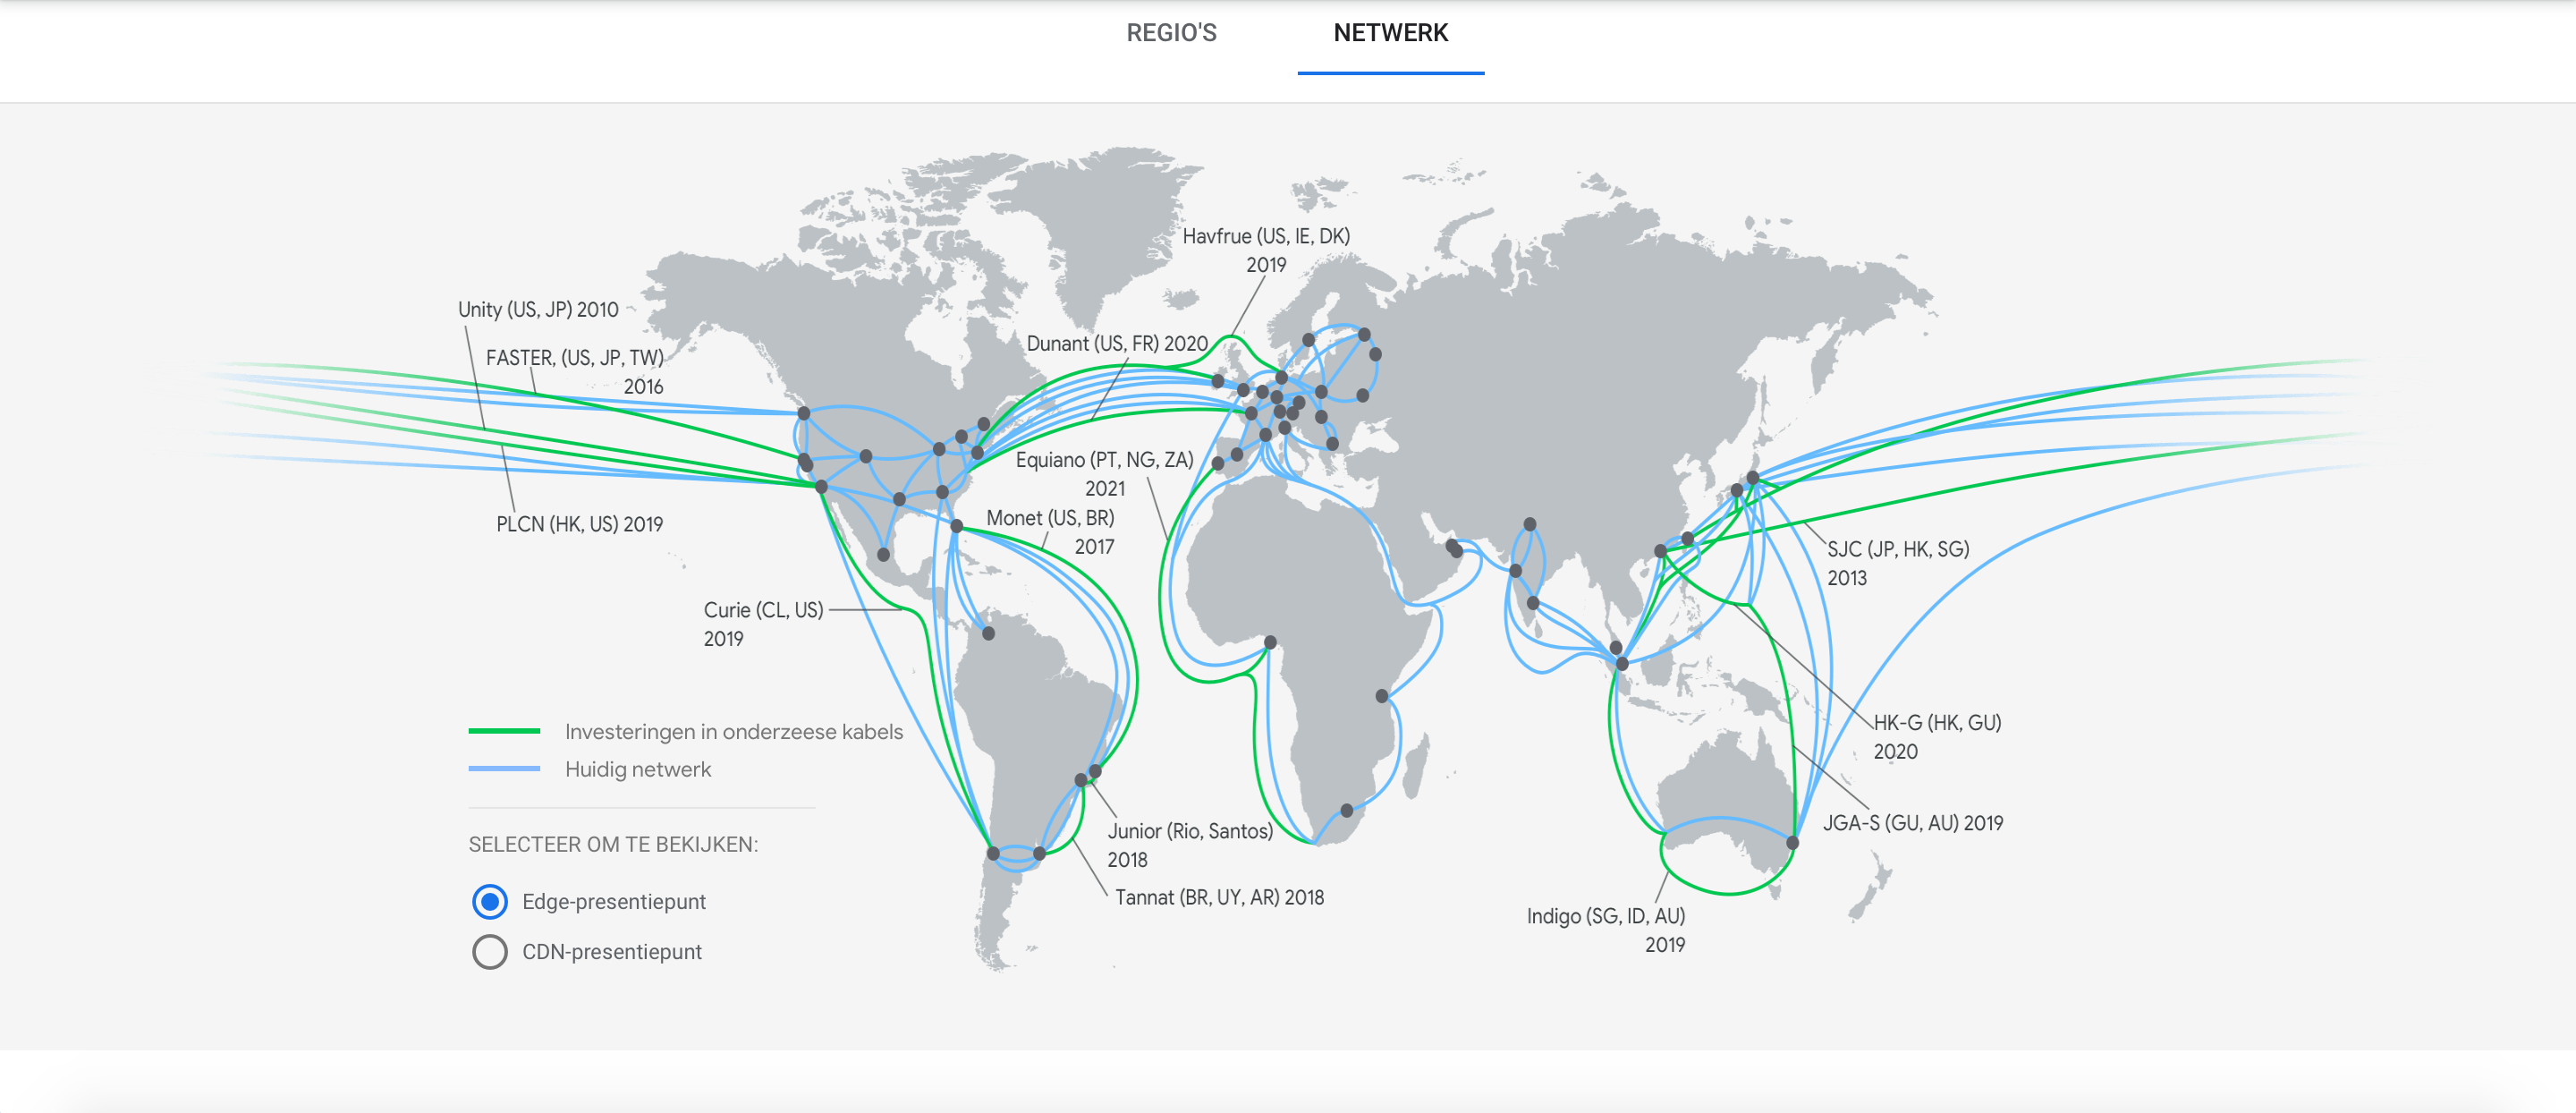
\includegraphics[width=\linewidth]{/Users/kenzie/Documents/HoGent/Bachelorproef/Images/GCP_NetwerkKaart.png}
    \caption{Overzicht van datacenter locaties Google Cloud. Figuur van \href{}{Google Cloud website}. Figuur toont de connectiviteit van de verschillende datacenters verspreid over de wereld.}
    \label{fig:GCP_NetwerkKaart}
\end{figure}

\begin{table}[!htbp]
    \begin{tabular}{|l|l|l|l|}
        \hline
        & Amazon AWS & Google Cloud & Azure DeVops \\ \hline
        Gespendeerde tijd in minuten & 195 & 125 & 60 \\ \hline
    \end{tabular}
    \caption{toont de gespendeerde tijd voor de gebruiksvriendelijkheid test per Cloud platform. De tijden staan in minuten. De Cloud platformen vergelijken goed met elkaar. Ook schaalt de complexiteit mee met de gespendeerde tijd.}
    \label{tab:gebruiksvriendelijkheid}
\end{table}